\documentclass[12pt,a4paper]{report}
\usepackage[utf8]{inputenc} % Set input encoding to UTF-8
\usepackage{eso-pic} % For background images
\usepackage[T1]{fontenc}    % Set font encoding to T1
\usepackage{lmodern}    % Use Latin Modern scalable fonts
\usepackage{xcolor}   % For colors
\usepackage{url}      % For formatting URLs
\usepackage{amsmath}  % For advanced mathematical typesetting
\usepackage{amssymb}  % For mathematical symbols
\usepackage{graphicx} % For including images
\usepackage{tikz}     % For creating diagrams
\usepackage{pgfplots} % For creating plots
\pgfplotsset{compat=1.18} % Set compatibility mode
\usetikzlibrary{positioning,arrows.meta,shapes.geometric,shapes.misc,decorations.pathreplacing,calc,shapes.arrows,backgrounds,fit}  % Additional TikZ libraries for Grover's diagram
\usepackage{booktabs} % For better tables
\usepackage{caption}  % For customizing captions
\usepackage{subcaption} % For subfigures and subcaptions
\usepackage{csquotes} % For better quotation handling
\usepackage{listings} % For code listings
\usepackage{etoolbox} % For environment hooks
% Temporarily commenting out unavailable packages - these might need to be installed in your LaTeX environment
% \usepackage{algorithm}   % For algorithms environment
% \usepackage{algpseudocode} % For pseudocode in algorithms
% \usepackage{physics}     % For physics notation
\usepackage{microtype}  % <-- UNCOMMENT THIS LINE
\usepackage[margin=1in]{geometry} % Setting document margins
\usepackage[
backend=biber, 
style=alphabetic, % Revert to original style
bibstyle=reading, % Revert to original bibstyle
sorting=nyt       % Revert to original sorting
]{biblatex} % For bibliography management with BibLaTeX and biber

% Declare the bibliography category *after* loading biblatex
% \DeclareBibliographyCategory{ytvideos} % REMOVE THIS

% Add ALL bib resources
\addbibresource{src/bibliography/ref.bib}
\addbibresource{src/bibliography/yt.bib}
% ... Add other bib resources here if needed ...

% Assign the specific resource to the category *after* adding it
% \assignresourcecategory{\bibdatamodel}{src/bibliography/yt.bib}{ytvideos} % REMOVE THIS

% Glossaries package
\usepackage[acronym,toc]{glossaries} % With acronym option and table of contents
\makeglossaries % Initialize glossaries
\loadglsentries{src/glossary} % REMOVED - Load individual files below


\loadglsentries{src/ch4_glossary_additions}
\loadglsentries{src/ch5_new_glossary_entries}
\loadglsentries{src/ch6_glossary_additions}
\loadglsentries{src/glossary_additions}
\loadglsentries{src/new_glossary_entries}


% Automatically add \noindent after list environments
\AfterEndEnvironment{itemize}{\noindent\ignorespaces}
\AfterEndEnvironment{}{\noindent\ignorespaces}
\AfterEndEnvironment{enumerate}{\noindent\ignorespaces}
\AfterEndEnvironment{description}{\noindent\ignorespaces}

% Configure hyperref for improved PDF navigation and appearance
\usepackage{hyperref} % For hyperlinks in the document
\hypersetup{
    colorlinks=true,       % Colors for links instead of boxes
    linkcolor=blue,        % Color of internal links
    filecolor=magenta,     % Color of file links
    urlcolor=cyan,         % Color of URLs
    pdftitle={Quantum Computing and Its Impact on Cryptography}, % PDF title metadata
    pdfauthor={Lou Sergonne},          % PDF author metadata
    pdfsubject={Thesis Subject},
    pdfkeywords={keyword1, keyword2},
    bookmarksopen=true,
    bookmarksnumbered=true,
    breaklinks=true
}

% Configure graphicx to search for images in both the root directory AND the src/images directory
\graphicspath{{./}{src/images/}}

% Remove "Chapter" from chapter headings
\renewcommand{\chaptername}{}

% Document title, author and date
\title{\LARGE{\textbf{Quantum Computing and Its Impact on Cryptography}}}
\author{\Large{Lou Sergonne}}
\date{2024-2025}

% Custom title page commands
\newcommand{\coverpage}{
  \begin{titlepage}
    \thispagestyle{empty}
    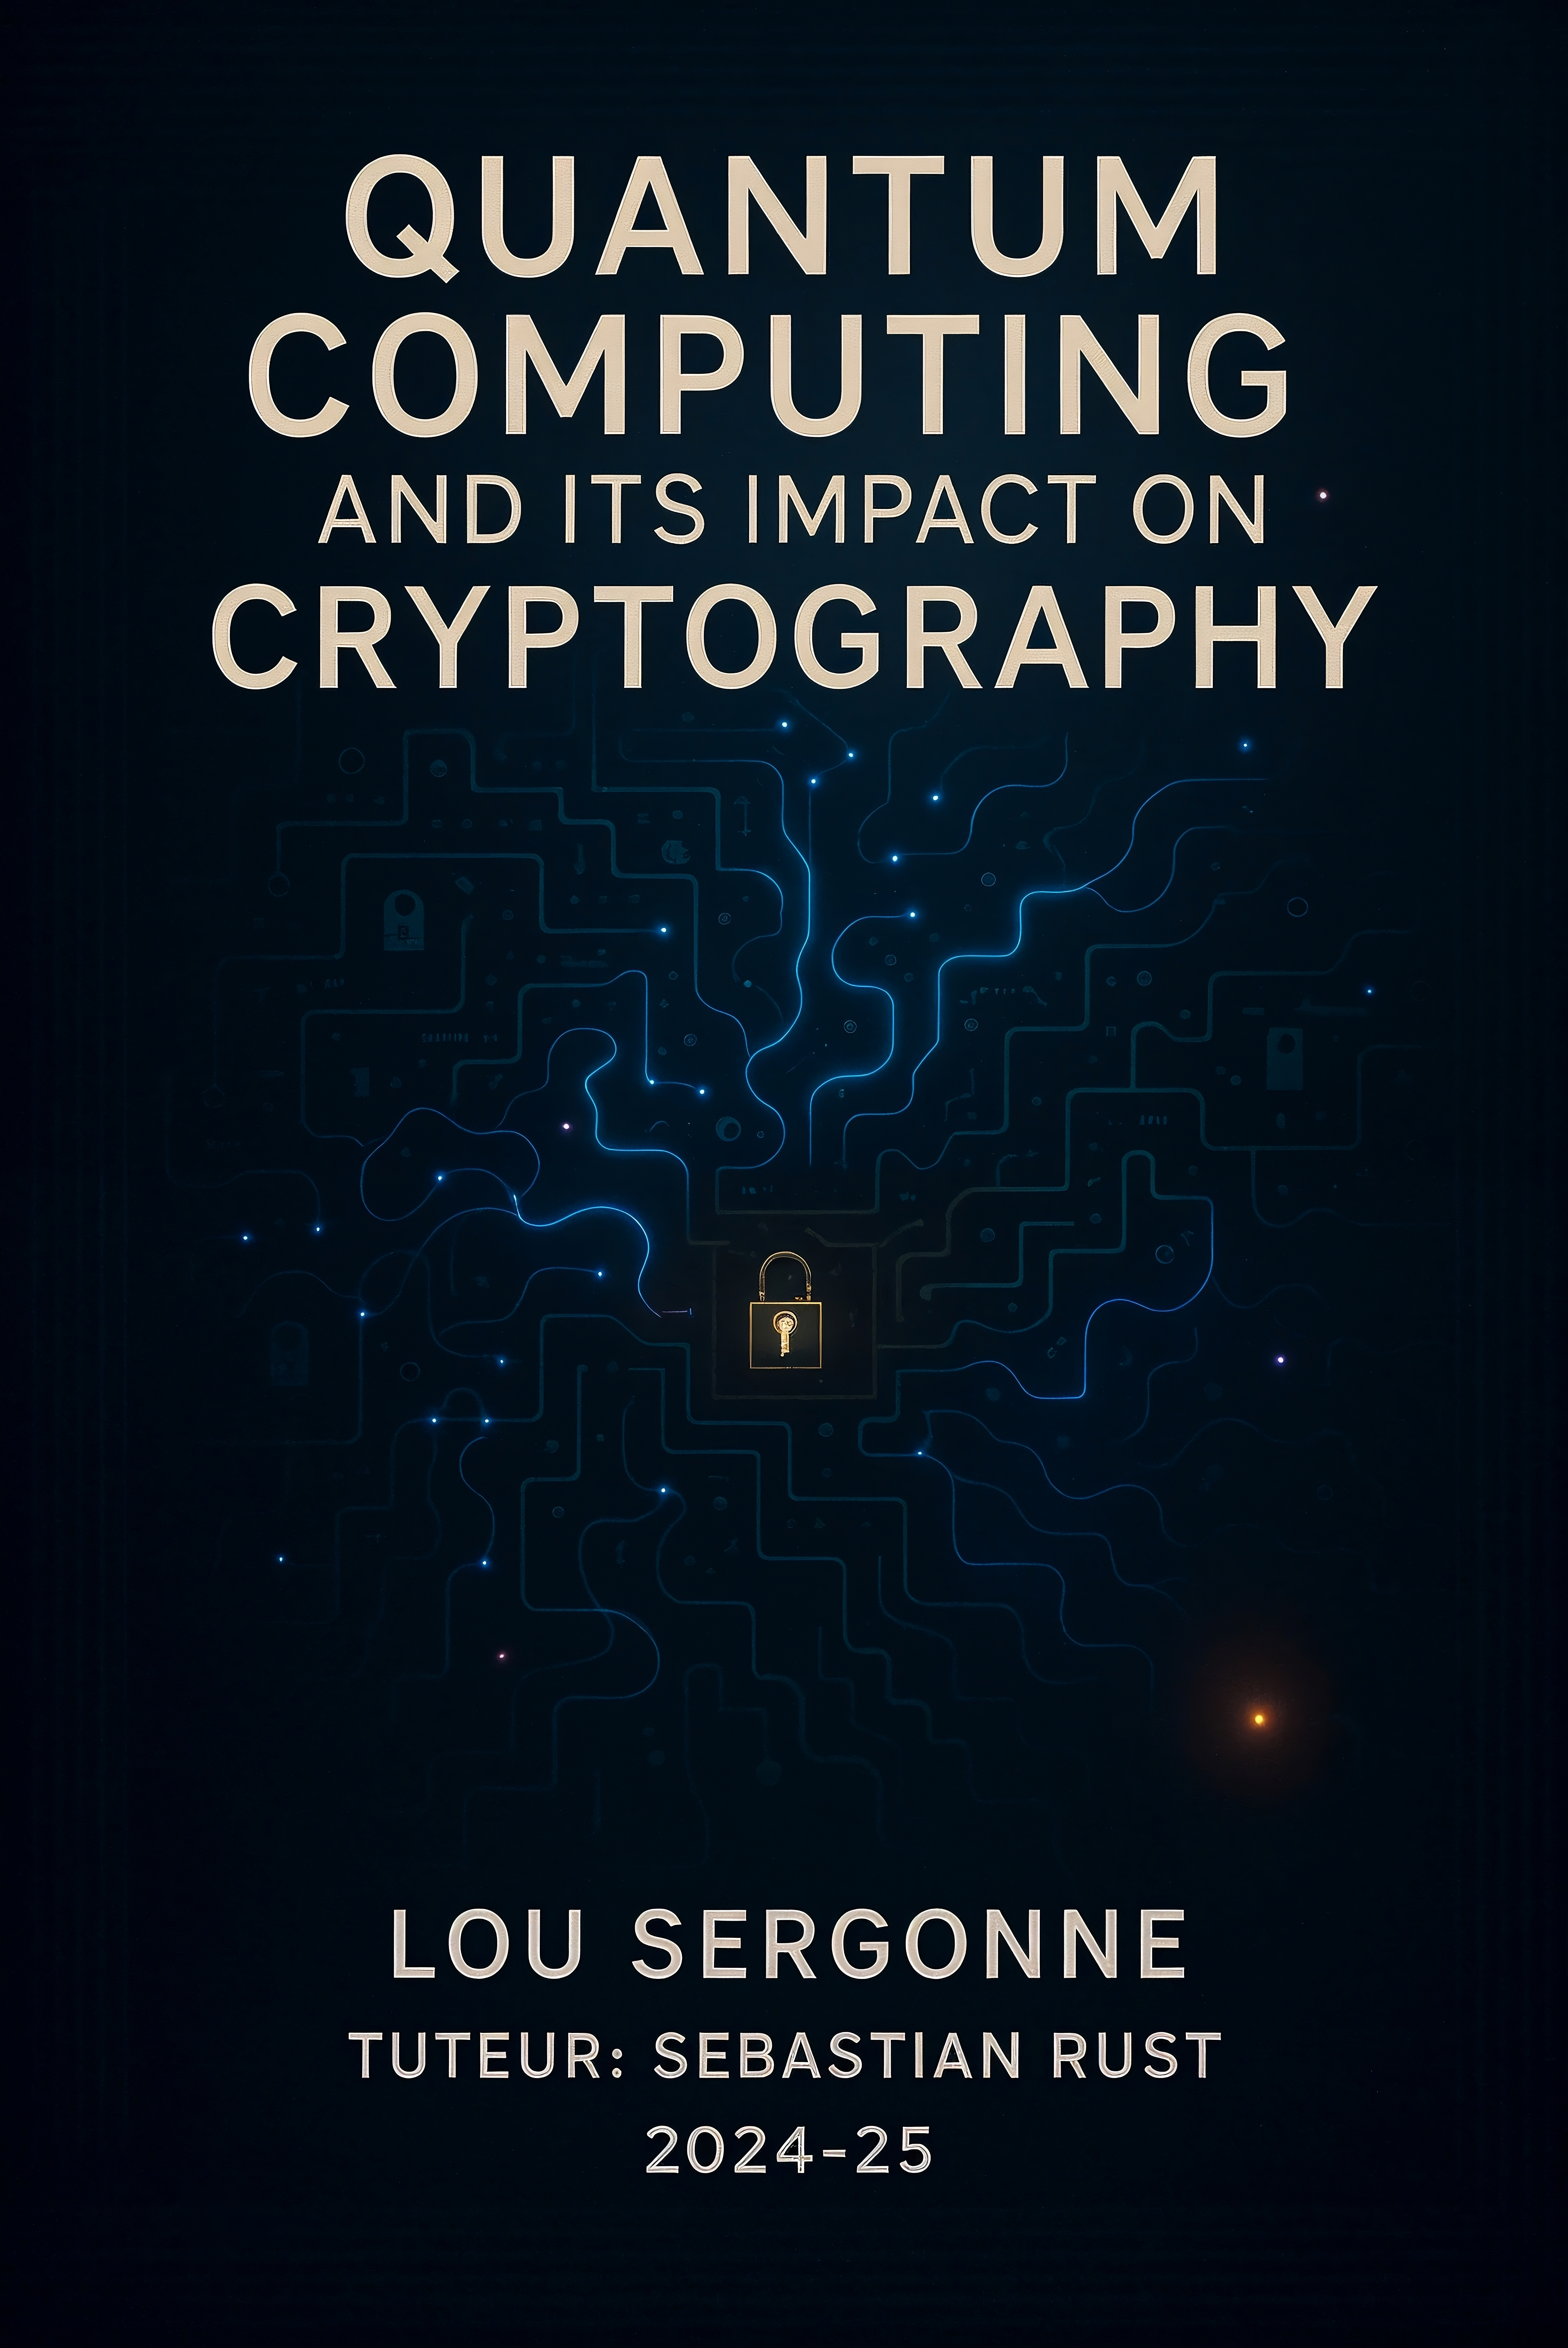
\includegraphics[width=\paperwidth,height=\paperheight]{upscalemedia-transformed.jpeg}
    \vspace*{-\paperheight}
    \begin{center}
      \vspace*{5cm}
      {\huge\bf \@title \par}
      \vspace{2cm}
      {\LARGE \@author \par}
      \vspace{1cm}
      {\large \@date \par}
    \end{center}
  \end{titlepage}
}

% Redefine \maketitle to use our custom coverpage
\renewcommand{\maketitle}{\coverpage}
